% -*- coding: utf-8 -*-

\documentclass[10pt,twocolumn,letterpaper]{article}

\usepackage{cvpr}
\usepackage{times}
\usepackage{epsfig}
\usepackage{graphicx}
\usepackage{amsmath}
\usepackage{amssymb}
\usepackage{subcaption}
\usepackage{textgreek}
\usepackage[numbers]{natbib}

% Allows for embedding of ancient Greek characters in document safely
\usepackage[utf8]{inputenc}
\usepackage[LGR,T1]{fontenc}

% Include other packages here, before hyperref.

% If you comment hyperref and then uncomment it, you should delete
% egpaper.aux before re-running latex.  (Or just hit 'q' on the first latex
% run, let it finish, and you should be clear).
\usepackage[breaklinks=true,bookmarks=false]{hyperref}

\cvprfinalcopy % *** Uncomment this line for the final submission

\def\cvprPaperID{****} % *** Enter the CVPR Paper ID here
\def\httilde{\mbox{\tt\raisebox{-.5ex}{\symbol{126}}}}

\newcommand\Koppa{\begingroup\fontencoding{LGR}\selectfont\char21\endgroup}

% Pages are numbered in submission mode, and unnumbered in camera-ready
%\ifcvprfinal\pagestyle{empty}\fi
\setcounter{page}{1}
\begin{document}

%%%%%%%%% TITLE
\title{Recognizing Ancient Greek Handwriting Using Modern Training Data}

\author{Sean Karlage\\
University of Kentucky\\
Lexington, KY\\
{\tt\small sean.karlage@uky.edu}
}
% For a paper whose authors are all at the same institution,
% omit the following lines up until the closing ``}''.
% Additional authors and addresses can be added with ``\and'',
% just like the second author.
% To save space, use either the email address or home page, not both

\maketitle
%\thispagestyle{empty}

%%%%%%%%% ABSTRACT
\begin{abstract}
    While recognition of machine-printed text with automated procedures is generally considered a solved problem by most computer scientists, recognition of handwriting is still a difficult problem in the field of computer vision. Recognition of ancient manuscript letterforms is made difficult due to document deformities, letterform occlusion, and general document age and all associated difficulties it brings.  There is a need for a classifier of ancient Greek letterforms extracted from ancient papyri; however, there is no known contemporary dataset of handwritten ancient Greek letterforms. Therefore, classifiers employing a variety of machine learning techniques were trained and cross-validated on the dataset proposed in \cite{GCDB} and tested on manually-segmented letterforms from the work of \cite{BYU}.
\end{abstract}

%%%%%%%%% BODY TEXT
\section{Introduction}

Automated recognition of machine-printed text is generally considered by some to be a solved problem in the field of computer vision. Many commercial and open-source systems exist that are designed to take as input images or scans of machine-printed text and output corresponding text elements with a high degree of accuracy. However, this automated process is much more difficult when it comes to recognizing handwritten text for a variety of reasons: different writing styles, various font embellishments, irregular line widths, and document medium irregularities, just to name a few.

Recognition of ancient handwritten text, in particular, represents a unique challenge in this field; in addition to the above-mentioned problems, texts can be malformed, occluded by foreign material on the document medium, or simply have degraded due to (sometimes exceptional) document age. The ability to recognize such text would be a distinct advantage for ancient document researchers, as they would be able to automatically extract letterforms that look promising for further study, as well as be able to more easily distinguish between actual letterforms and random noise in the document medium. Furthermore, experts knowledgable about that particular document's contents would not be required for initial analysis of whether a letterform is valid.

%-------------------------------------------------------------------------
\subsection{Motivation}

As a part of the larger “volume cartography” project occurring at \cite{VisCenter}, a need arose for automated recognition of ancient Greek handwritten letterforms.  Because the volume of data that could potentially contain text is large, manually parsing flattened, textured volume data for possible letterforms is infeasible. Furthermore, in addition to team member validation, professional analysis from experts in ancient Greek writings would be required in order to evaluate and validate any potential discoveries.

As a first pass, however, automated recognition of potential letterforms provides a good estimate of signal-to-noise ratio and evaluation of letterform extraction procedures. To the author’s knowledge, however, no open or commercial database of segmented ancient Greek handwritten letterforms exists with which to serve as a training dataset for any potential text classification algorithm. Instead, the author proposes to train classifiers based on datasets of modern Greek handwriting - in particular, the dataset proposed in \cite{GCDB} - and evaluate the classifier on letterforms extracted by hand from the document corpus of \cite{BYU}. This corpus is comprised of documents taken from ancient papyrus scrolls from Herculaneum, Petra, and the Judean Desert \cite{chabries2003imaging}. An example of an extracted letterform is in \ref{fig:regalpha}.

\subsection{Datasets}

The ancient and modern Greek alphabets are nearly identical, with the exception of three letters that have fallen out of use, due either to redundancy or disuse of that particular sound in the spoken language: F $($\textit{digamma}$)$, M $($\textit{san}$)$, and \Koppa$\:($\textit{koppa}$)$. As such, these letters are excluded from testing in the evaluation section. Ancient Greek manuscripts were also traditionally written in all capital letters.

The dataset presented in \cite{GCDB} is a small part of a larger system devoted to collecting modern Greek handwriting samples from many different people. The database developed by the authors was built with an eye toward extensibility and flexibility, retaining information such as gender and age of the text sample authors, and collecting samples not only of individual letters, but also entire words to allow for handwriting analysis at the word and phrase level. Only uppercase letters are considered for the work presented here. All letterforms from GCDB are binarized and were resized to $49$x$51$ pixels. An example of a \textAlpha$\:$ is presented in \ref{fig:malpha}.

Letterforms were extracted from the corpus of \cite{BYU} by hand with the use of Photoshop. Images were loaded into the program and then individually segmented and classified by a researcher from \cite{VisCenter}. The extracted letterforms comprise almost all letters in the ancient Greek alphabet, with the exception of Ξ $($\textit{chi}$)$ and Ψ $($\textit{psi}$)$; as such, the corresponding letters from the dataset presented in \cite{GCDB} were excluded from the training component for all classifiers. The segmented letters were binarized by first transforming them into grayscale images and then performing a threshold. They were then resized to $49$x$51$ pixels to match samples from GCDB. There are approximately 150 "good" letterforms - those that both survived the process of being transformed to grayscale images and that still had suitable structure after binarization. The structure of the binarized letterforms are still quite rough, as can be seen in \ref{fig:binalpha}. There is a lot of noise present in some of the binarized images, as can be seen in \ref{fig:noisyLambda}. These approximately 150 letterforms served as the final testing dataset for the letter classifiers.

\begin{figure}
    \centering
    \begin{subfigure}{0.5\textwidth}
        \centering
        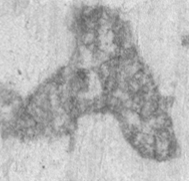
\includegraphics[width=0.4\linewidth]{res/198423984.png}
        \caption{Extracted letterform of an ancient Greek \textAlpha}
        \label{fig:regalpha}
    \end{subfigure}
    \begin{subfigure}{0.5\textwidth}
        \centering
        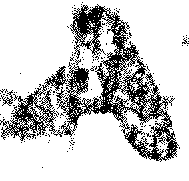
\includegraphics[width=0.4\linewidth]{res/001.png}
        \captionof{figure}{The letterform of \ref{fig:regalpha} binarized}
        \label{fig:binalpha}
    \end{subfigure}
    \begin{subfigure}{0.5\textwidth}
        \centering
        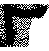
\includegraphics[width=0.4\linewidth]{res/002.png}
        \caption{Extremely noisy example of an extracted \textLambda$\:$ from the corpus of \cite{BYU}}
        \label{fig:noisyLambda}
    \end{subfigure}
    \begin{subfigure}{0.5\textwidth}
        \centering
        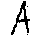
\includegraphics[width=0.4\linewidth]{res/form14.png}
        \caption{Modern handwritten Greek \textAlpha$\:$ from \cite{GCDB}}
        \label{fig:malpha}
    \end{subfigure}
\end{figure}



%------------------------------------------------------------------------
\section{Related Work}

Automated recognition of letters from Early Christian Greek manuscripts has been carried out previously in \cite{segFree}, in which the authors employed a segmentation-free approach by detecting open and closed cavities in letterforms and using those as a basis with which to extract features of each character. The system developed by the authors obtained a recall value of 89\% for simple letterforms in their testing dataset.

The HisDoc project \cite{HisDoc} involved not only handwriting recognition and digitization of manuscript text data, but also developing an information retrieval system around recovered data. The authors developed this system and applied it primarily to three text corpora in different languages (Latin, German, and English). Their system accurately segmented and recognized text from each corpus and, using a neural network-based approach, had word recognition error rates of less than 10\%.

The authors of \cite{Diem1} also proposed a segmentation and binarization-free approach to recognizing letterforms from ancient Slavonic documents using SIFT features, SVM classifiers, and finally a weighted voting algorithm based on pre-classified local descriptors. Disregarding binarization of input images allowed for their classifiers to work with more data from each letterform, particularly those that were heavily degraded or experienced severe occlusion from stains or tears in the manuscript. Affine transformations were also applied to sample selections from documents in order to determine the resiliency of the authors' extracted and local features used at the end of their proposed method. It was found that SIFT features performed the best overall in the classification task with affine transformations induced.

The authors of \cite{GRUHD} were the first to develop an open dataset of modern Greek handwriting that contained extensive metadata about participants, as well as providing very well-segmented letterforms and words from each individual author. The sample text contains simple Greek words as well as both uppercase and lowercase Greek letters and numerals from 1000 individual contributors. This database has been supplanted by the work of \cite{GCDB}, from the same authors, with improvements to database architecture and archival. GCDB also contains Greek word samples and letterforms from 305 unique contributors.

%-------------------------------------------------------------------------
\section{Problem Statement}

With the lack of ancient Greek handwriting datasets, building and evaluating a detector on live data proves difficult. In order to approximate a recognition system, we propose to answer the following primary research question:

\begin{quote}
    \textit{Can a handwriting recognition system that is trained on modern Greek handwriting be used to classify segmented letterforms from ancient Greek manuscripts?}
\end{quote}

Two forms of classifiers, k-Nearest Neighbors and Support Vector Machines, will be built that will be validated against the training dataset and tested against live data from the corpora of \cite{BYU}.

%-------------------------------------------------------------------------
\section{Approach}

Uppercase letterforms retrieved from the GCDB database will comprise the training dataset. There are 9,910 images in the testing dataset, with an approximately uniform distribution across all letters. As mentioned previously, due to the lack of the letters \textPsi$\:$ and \textXi$\:$ in the testing dataset they are excluded from the training set. Scikit-learn \cite{scikit-learn} was used to develop all code, as it provides a rich set of libraries with which to develop and validate many different kinds of classifiers. In order to get a variety of results from training data, two classifiers were developed: one using the k-nearest neighbors classification algorithm, and the other using the support vector machine algorithm. In order to accurately train and validate the classifier, 50\% of the samples from GCDB were used for the training dataset, while the other half was used to perform cross-validation. Finally, the classifier was tested with the 150 letterforms extracted from the corpus of \cite{BYU}.

%-------------------------------------------------------------------------
\subsection{k-Nearest Neighbors with PCA}

First, a k-nearest neighbor classifier was constructed to classify the data. Principle Component Analysis was utilized to reduce the dimensionality down from 2500 (the number of pixels in each input image). It was found that $60$ was the optimal number of dimensions for PCA. Scaling was utilized to bring all reduced dimensional components into a common scale. Results from this method are presented in the evaluation section.

%-------------------------------------------------------------------------
\subsection{SVM with PCA}

A support vector machine was trained on the training data, again with a 50/50 split in terms of train/validation ratio. Again principle component analysis was used to reduce the dimensionality of input data. The optimal number of dimensions for PCA was found to be $60$ as well. Afterward, scaling was again used to bring all features into a common scal. In order to optimize the parameters of the SVM classifier, an exhaustive grid search was performed that iterated over different kernels, values of $C$ and $\gamma$. The optimal classifier was found to occur with a kernel function of
\begin{align*}
    f(x) = e^{-\gamma \left| x - x' \right|^2}
\end{align*}
and the optimal values of $C$ and $\gamma$ were found to be $10$ and $0.01$, respectively.

%-------------------------------------------------------------------------
\section{Evaluation}
\subsection{k-Nearest Neighbors with PCA}

The simple k-Nearest Neighbors classifier was evaluated on the GCDB dataset. Through experimentation, the optimal value of $k$ was found to be 10. This yielded a cross-validation percentage of only $38.6\%$. However, when evaluated on the testing dataset, the highest percentage seen, $8.0\%$, was the overall highest observed not only for different values of both $k$ and the number of dimensions obtained through PCA, but also out of all classifiers used in the study.

\subsection{SVM with PCA}
The SVM classifier utilizing principal component analysis obtained a classification accuracy of $54.3\%$ on the cross-validation test. This was the highest-observed accuracy for the parameters given in section 4. Compared to the k-nearest neighbors with PCA, this method did far better in the cross-validation testing. However, when run with the real data, the classifier was only able to achieve $5.7\%$. Additionally, it was observed that the classifier simply guessed a constant value for every sample in the testing dataset. The confusion matrix for the cross-validation step can be observed in Table \ref{tab:confmatrix}.

\begin{table}
    \centering
    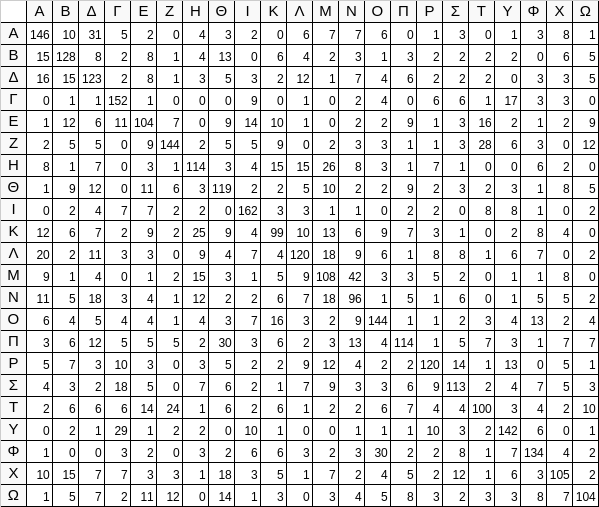
\includegraphics[width=0.4\textwidth]{res/table1.png}
    \caption{Confusion matrix for SVM classifier}
    \label{tab:confmatrix}
\end{table}

%-------------------------------------------------------------------------
\section{Discussion}

As can be seen from the results obtained from both the k-nearest neighbors and support vector machine classifiers, the accuracy of both methods leaves something to be desired. The cross-validation scores of both classifiers are quite low compared to other character recognition systems, although remarkably the cross-validation score of the SVM classifier achieved a somewhat acceptable accuracy of 54.3\%. However, while this problem space is difficult given the extreme variability of handwriting across the scores of people sampled in the GCDB collection, it is the opinion of the author that this cross-validation score could be much higher for both classifiers.

The accuracy of the classifiers when tested against the letterforms from the corpus of \cite{BYU} is also incredibly poor. Simply guessing a consistent class for each testing sample would yield around the same percentage as obtained with the SVM classifier (and indeed, this is exactly what the classifier ended up doing). There remains room for much more optimization in this area, as well as experimentation with different extracted features from each input image. Furthermore, extending the types of classifiers and in combining them in different ways may lead to higher accuracy. For example, utilizing a large neural network with sufficient training data augmentation and feeding the output to a logistic regression component. Additionally, more pre-processing of the ancient Greek letterforms will be required. The minimal pre-processing of data discussed here introduced many image deformities that more than likely contributed to the poor performance of the classifiers.

Two classification algorithms were trained on modern Greek handwriting samples and tested on ancient Greek handwritten letterforms extracted from ancient documents. There are still many optimizations to be performed on these classifiers and others in order to achieve suitable accuracy when used against unknown data. The cross-dataset validation problem for classification algorithms is already quite tough; combined with the variability of raw handwriting data, the problem becomes even more difficult, but much more interesting.

%-------------------------------------------------------------------------
\newpage
{\small
\bibliographystyle{ieee}
\bibliography{egbib}
}

\end{document}
